% =====================================================================
% ejercicio06.tex
% Responsabilidad única: explorar el caso diabetes en entrenamiento, ajustar la regresión simple
% con \texttt{bmi} (NumPy y scikit-learn), compararla con el predictor
% constante y analizar residuos de validación.
% Las cifras provienen de generado/resultados.tex y generado/tabla_*.tex.
% =====================================================================
\subsection{Ejercicio 6: Caso A, regresión lineal simple y modelo de referencia}
% Holgura extra para párrafos con nombres largos en \texttt (rige en 6-10).
\setlength{\emergencystretch}{2.5em}

\begin{enumerate}

\item \textbf{Exploración en entrenamiento.}
Lo primero que revisamos fue el tipo y los faltantes de cada columna: los
diez predictores son numéricos (\texttt{float64}) y no tienen valores
faltantes en entrenamiento, al igual que la variable objetivo
(Tabla~\ref{tab:ex6-exploracion}), así que no tuvimos que imputar nada. Como
cargamos los datos con \texttt{scaled=False}, las variables quedaron en sus
unidades originales y con rangos muy distintos (por ejemplo \texttt{s1} en
cientos y \texttt{s5}, el logaritmo de los triglicéridos, en unidades), y
\texttt{sex} es binaria codificada como 1 y 2. La variable objetivo es una
medida cuantitativa de progresión cuya unidad no documenta scikit-learn, por
lo que en adelante hablamos de unidades de la escala del \emph{target}.

\begin{table}[H]
\centering
\small
% Archivo generado automáticamente por el notebook (no editar a mano).
\begin{tabular}{lrrrrr}
\toprule
Variable & Faltantes & Mínimo & Máximo & Media & Desv. est. \\
\midrule
age & 0 & 19.00 & 79.00 & 48.84 & 12.77 \\
sex & 0 & 1.00 & 2.00 & 1.49 & 0.50 \\
bmi & 0 & 18.90 & 41.30 & 26.49 & 4.38 \\
bp & 0 & 62.00 & 126.00 & 94.31 & 14.03 \\
s1 & 0 & 110.00 & 301.00 & 187.47 & 35.29 \\
s2 & 0 & 41.60 & 242.40 & 114.61 & 31.30 \\
s3 & 0 & 22.00 & 98.00 & 48.85 & 12.30 \\
s4 & 0 & 2.00 & 9.09 & 4.09 & 1.27 \\
s5 & 0 & 3.58 & 6.11 & 4.65 & 0.50 \\
s6 & 0 & 58.00 & 124.00 & 92.35 & 11.42 \\
target (y) & 0 & 25.00 & 346.00 & 149.81 & 79.00 \\
\bottomrule
\end{tabular}

\caption{Faltantes y rangos de los predictores y de la variable objetivo (entrenamiento).}
\label{tab:ex6-exploracion}
\end{table}

En la Figura~\ref{fig:ex6-bmi} vimos una tendencia creciente con amplia
dispersión vertical (correlación de Pearson de $\CorrBmiTarget$), de forma
que una recta es una aproximación razonable para la tendencia promedio
aunque deja buena parte de la variabilidad sin explicar, y además nos dio la
impresión de que la nube se abre un poco para valores altos de
\texttt{bmi}. No eliminamos ninguna observación, pues los puntos alejados
son plausibles y nada indica errores de registro.

\begin{figure}[H]
    \centering
    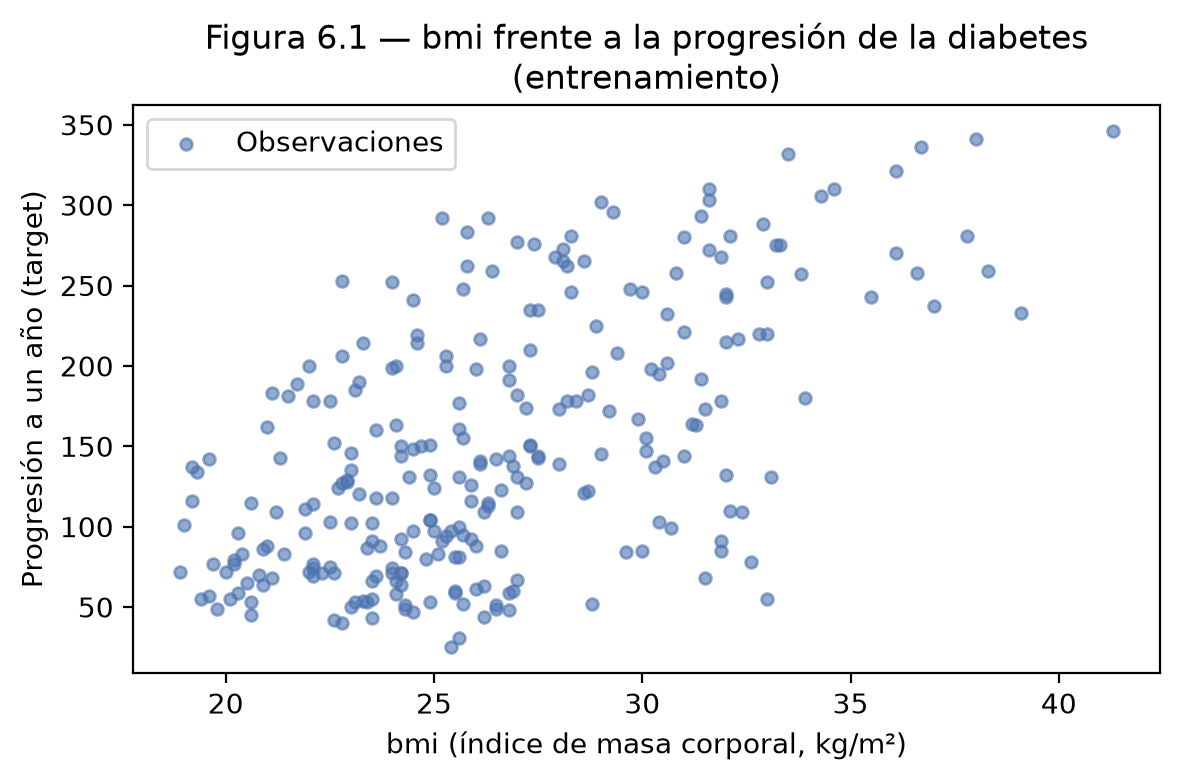
\includegraphics[width=0.68\textwidth]{figuras/ex6_bmi_target.png}
    \caption{\texttt{bmi} frente a la progresión de la diabetes (entrenamiento).}
    \label{fig:ex6-bmi}
\end{figure}

\item \textbf{Implementación con NumPy vs.\ \texttt{LinearRegression}.}
Aplicando a \texttt{bmi} las mismas expresiones que derivamos en el
Ejercicio~1 obtuvimos $\hat\beta_0 = \SimpleBetaCero$ y
$\hat\beta_1 = \SimpleBetaUno$, los mismos coeficientes que reporta
\texttt{LinearRegression}, y la diferencia absoluta máxima entre las
predicciones de validación de ambas implementaciones fue de
$\SimpleDifMax$, es decir, error de redondeo de punto flotante, por lo que
\texttt{np.allclose} devolvió \texttt{True}. Con esto nos quedó claro que,
con un solo predictor, scikit-learn resuelve exactamente el mismo problema
de mínimos cuadrados que hicimos a mano, solo que mediante una
factorización numérica en lugar de las sumas explícitas.

\item \textbf{Comparación con \texttt{DummyRegressor}.}

\begin{table}[H]
\centering
\small
% Archivo generado automáticamente por el notebook (no editar a mano).
\begin{tabular}{llrrr}
\toprule
Modelo & Partición & MAE & RMSE & $R^2$ \\
\midrule
Constante (media) & Entrenamiento & 66.6773 & 78.8462 & 0.0000 \\
Constante (media) & Validación & 64.1288 & 75.6392 & $-$0.0443 \\
Regresión simple (bmi) & Entrenamiento & 51.5459 & 63.3458 & 0.3545 \\
Regresión simple (bmi) & Validación & 50.3475 & 58.5671 & 0.3739 \\
\bottomrule
\end{tabular}

\caption{Predictor constante frente a regresión simple (entrenamiento y validación).}
\label{tab:ex6-comparacion}
\end{table}

La regresión simple mejoró las tres métricas frente al predictor constante
en ambas particiones (Tabla~\ref{tab:ex6-comparacion}): en validación el
RMSE bajó de $\RegDummyRMSEVal$ a $\RegSimpleRMSEVal$ y el MAE de
$\RegDummyMAEVal$ a $\RegSimpleMAEVal$, mientras que $R^2$ pasó de
$\RegDummyRdosVal$ a $\RegSimpleRdosVal$, de modo que \texttt{bmi} por sí
solo explica cerca de un tercio de la variabilidad en validación. El $R^2$
negativo de la constante al principio nos extrañó, pero no es un error: la
media se estima con entrenamiento y el $R^2$ de validación se mide contra la
media de validación, por lo que cualquier desfase entre ambas lo vuelve
ligeramente negativo, y en todo caso ninguna métrica empeoró con la
regresión simple. Algo que sí anotamos desde aquí es que los dos modelos
(incluida la constante) tuvieron menor error en validación que en
entrenamiento, lo que apunta a una partición de validación algo más
favorable y no a un fenómeno propio del modelo.

\item \textbf{Residuos de validación.}
Los residuos (Figura~\ref{fig:ex6-res}) se distribuyen alrededor de cero sin
una curvatura marcada, pero su dispersión crece con el valor predicho
(desviación estándar de $\ResStdBaja$ en la mitad de predicciones bajas
frente a $\ResStdAlta$ en la mitad alta), lo que nos hizo sospechar
heterocedasticidad, y hay errores grandes en ambos sentidos (entre $\ResMin$
y $\ResMax$). Esto implica que el RMSE resume un error que en realidad es
menor para pacientes con \texttt{bmi} bajo y mayor para \texttt{bmi} alto,
que los errores estándar clásicos de mínimos cuadrados (que suponen varianza
constante) no serían confiables para inferencia y que, con tanta dispersión
residual, faltan predictores. Eso fue lo que nos llevó al modelo múltiple
del Ejercicio~7.

\begin{figure}[H]
    \centering
    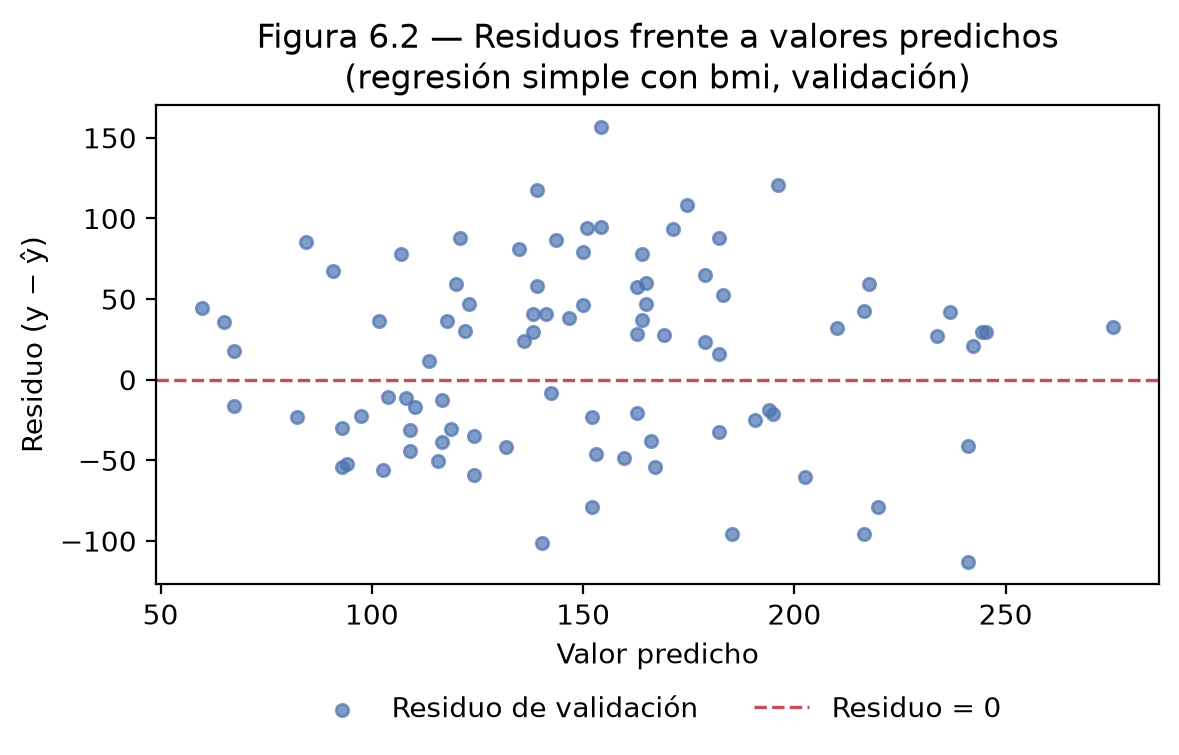
\includegraphics[width=0.68\textwidth]{figuras/ex6_residuos.png}
    \caption{Residuos frente a valores predichos de la regresión simple (validación).}
    \label{fig:ex6-res}
\end{figure}

\item \textbf{Interpretación de coeficientes y causalidad.}
El intercepto ($\SimpleBetaCero$) es la predicción para \texttt{bmi} igual
a cero, valor fuera del rango observado (Tabla~\ref{tab:ex6-exploracion}),
por lo que solo ubica la recta y no le dimos lectura práctica, mientras que
la pendiente ($\SimpleBetaUno$) indica que cada kg/m$^2$ adicional de
\texttt{bmi} se asocia, en promedio, con $\SimpleBetaUno$ unidades más de
progresión predicha. Esta asociación no identifica el efecto de intervenir
sobre \texttt{bmi}, pues los datos son observacionales y \texttt{bmi} se
relaciona con otros factores (presión arterial, lípidos, edad) que también
influyen en la progresión, de modo que la pendiente mezcla el efecto propio
de \texttt{bmi} con el de esas variables. De hecho, cuando pasamos al modelo
múltiple del Ejercicio~7 la pendiente equivalente bajó a unas
$\BmiPorUnidad$ unidades por kg/m$^2$.

\end{enumerate}
